\chapter{Camera Lens Calibration} \label{chap:Camera Lens calibration}

\noindent A calibration algorithm that iterativly determines the distortion coefficient was developed. This chapter presents a detail explanation of how it workd. A summary of the results can be seen in Figure \ref{fig:distortion}.

\noindent Virtual images were used for experimentation. These where created using $R^3$ software with known distortion coefficients. 
These images were recreated from the results of a previous calibration done manually at wTVision to ensure realistic values. The 
obtained images where saved in a folder. In this folder, there were images with different zoom and focus levels.
For a specific zoom and focus level, for example Zoom 0 and Focus 0, there were four images, one for each distortion coefficient
that needs to be determined: Center-shift\footnote{Note that even though there is an image for calibrating the center-shift at each level, this is not necessary since for calibrating the center-shift only the zoom matters. In fact, only the images at zoom 0 and at maximum zoom are required. In other words, the same center-shift calibration results can be obtained using images captured at a zoom level of 0 with any focus value within its minimum and maximum range, and another image taken at the maximum zoom level with a focus value.}, \ac{FoV}, K1 and K2.

\noindent The objective is to accuratly determine the distortion coefficients of the (simulated) images. The distortion coefficients are then compared to the real values to evaluate the accuracy of the calibration process.

\noindent Before initiating the calibration process, it is essential to measure the dimensions and position of the real target. The origin of the real-world coordinate system is defined at floor level, directly below the camera's optical point. Using these measurements, a virtual object is inserted into the \( R^3 \) software. Additionally, the pan, roll, and tilt of the camera must all be set to zero.

\section{Center-shift calibration} \label{sec:Center-shift calibration}

\noindent A program capable of accurately detecting the corners of the target in the real world has been developed. In this step the \( R^3 \) software is used to incorporate a virtual object with the same pattern as the real-world target, using the image captured by the camera, to calibrate the center-shift.

\noindent At this stage, a virtual target with accurate dimensions is present in the virtual environment. The first step in the calibration process is determining the center-shift. Experimental validation of the existing calibration procedure has demonstrated that when the camera’s tilt, pan, and roll are set to zero, the center-shift values correspond precisely to the pixel coordinates of the center of the light circle. This conclusion was derived through manual calibration of the center-shift and by using the edge detection program to identify the coordinates of the light circle’s center.

\noindent The center-shift calibration procedure follows a systematic approach. Initially, the camera is set to its minimum zoom level, and the target is positioned at the center of the frame. The image is then focused, and the edge-detection program is utilized to determine the coordinates of the center point. These coordinates are subsequently updated as the new center-shift values. The camera zoom is then adjusted to its maximum level, and the target is refocused to verify the accuracy of the center-shift calibration.

\noindent The center-shift calibration process is illustrated in Figure \ref{fig:main}. The real object is shown in Figure \ref{fig:a}, with the red square representing the target. In Figure \ref{fig:b}, a virtual cone is inserted into the \( R^3 \) software with an uncalibrated center-shift. The center coordinates of the real object are detected in Figure \ref{fig:c}, and the virtual cone is calibrated in Figure \ref{fig:d}. The final result is shown in Figure \ref{fig:f}, with the virtual cone correctly calibrated to the real object. \ref{fig:f} shows the result of changing the pan, tilt and/or roll of an already calibrated center-shift.

\begin{figure}[h]
    \centering
    \begin{subfigure}[b]{0.45\textwidth}
        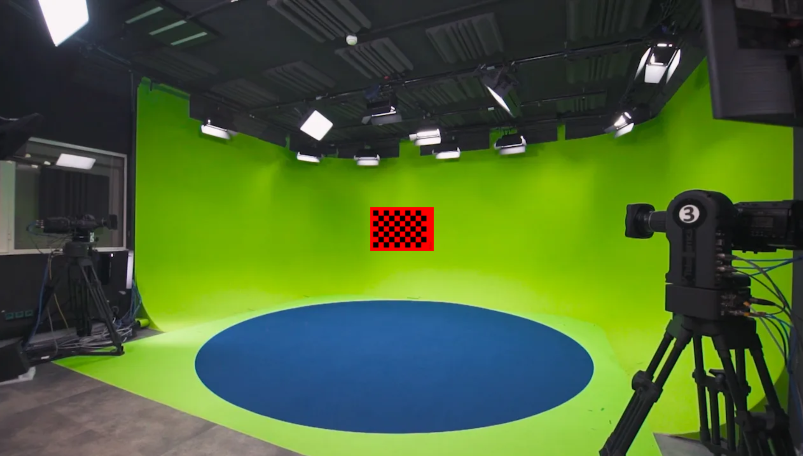
\includegraphics[width=\textwidth]{Images/04calibration/1.png}
        \caption{}
        \label{fig:a}
    \end{subfigure}
    \hfill
    \begin{subfigure}[b]{0.45\textwidth}
        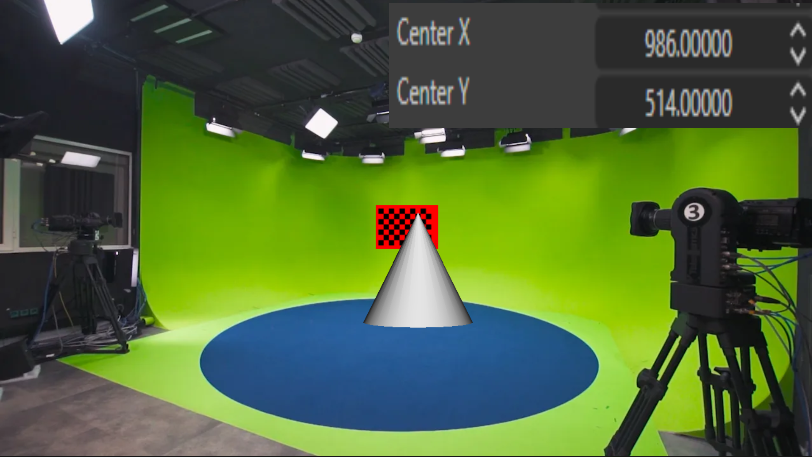
\includegraphics[width=\textwidth]{Images/04calibration/2.png}
        \caption{}
        \label{fig:b}
    \end{subfigure}
    
    \vspace{0.5cm}
    
    \begin{subfigure}[b]{0.45\textwidth}
        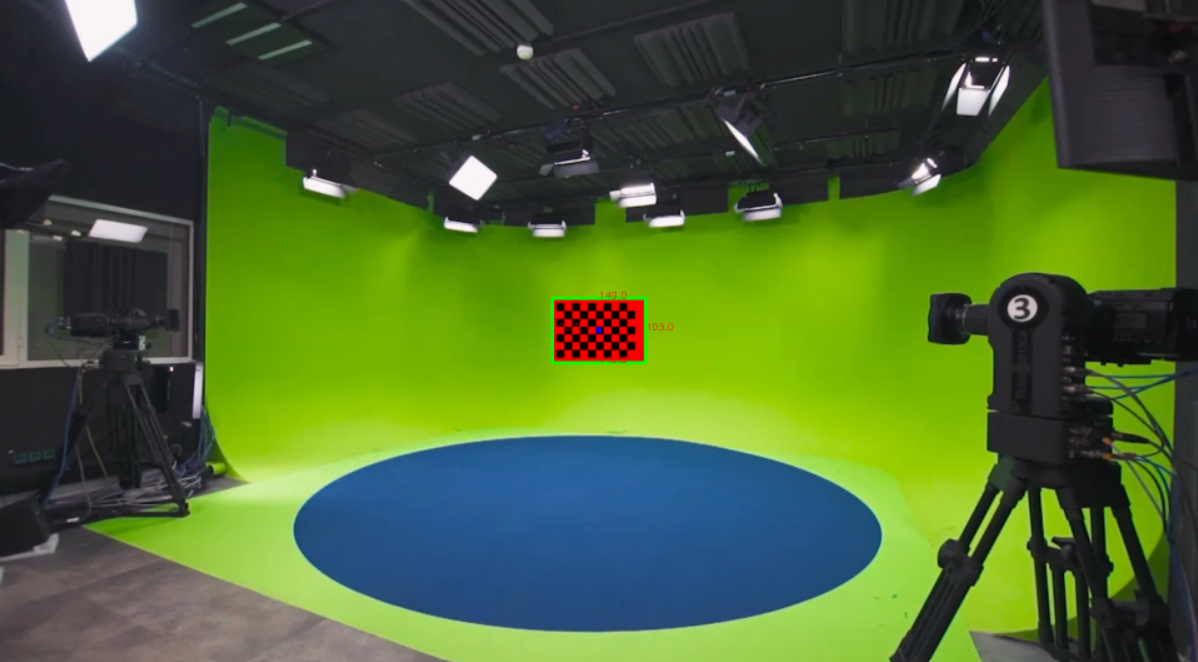
\includegraphics[width=\textwidth]{Images/04calibration/3.png}
        \caption{}
        \label{fig:c}
    \end{subfigure}
    \hfill
    \begin{subfigure}[b]{0.45\textwidth}
        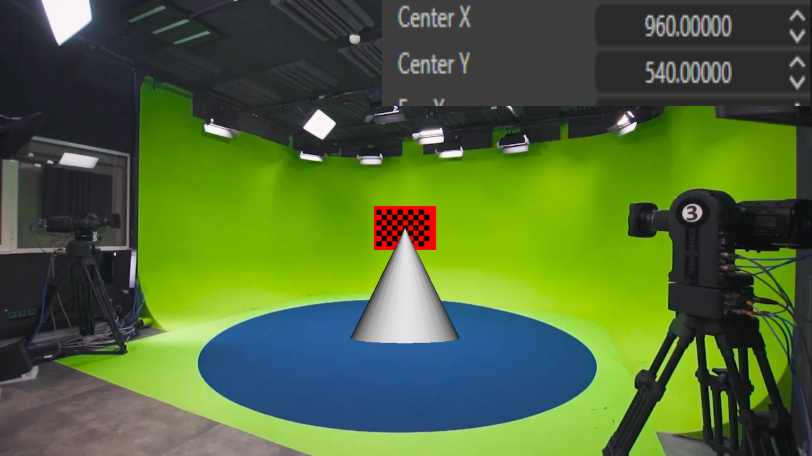
\includegraphics[width=\textwidth]{Images/04calibration/4.png}
        \caption{}
        \label{fig:d}
    \end{subfigure}

    \caption{Example of a center-shift calibration:(a) - Real object (red square) at max zoom, (b) - Insertion of a virtual cone with uncalibrated center-shift, (c) - Detection real object center coordinates, (d) - Calibrated virtual cone.}
    \label{fig:main}
\end{figure}

\begin{figure}[h]
    \centering
    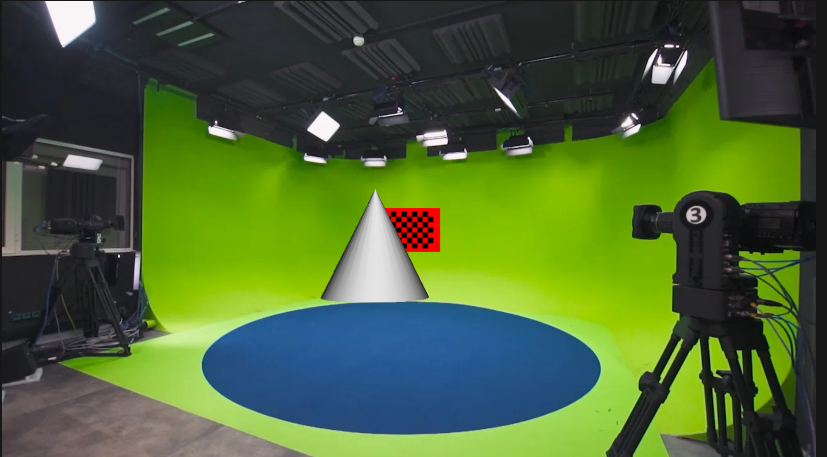
\includegraphics[width=0.45\textwidth]{Images/04calibration/5.png}
    \caption{calibrated center-shift after changing the pan and tilt}
    \label{fig:f}
\end{figure}

\section{ K1, K2 and \ac{FoV} calibration} \label{sec:FoV calibration}

\noindent Following this, the calibration of the \ac{FoV} is performed. The procedure involves applying a pan movement 
to the camera, causing the target to shift laterally within the frame. The edge-detection program is 
then employed to extract the edges of the real target like shown in figure \ref{fig:fov_cal}. Then the background is 
then turned off and the virtual object is inserted, for each iteration the program detectes the corners of the virtual object\footnote{This means that the $R^3$ software has to take and save a snapshot for each iteration. These snapshots are saved and rewritten into the disk which constituites a big limitations in terms of time efficiency.} like shown in 
figure \ref{fig:vir_fov_cal}.  
It has been observed that the virtual object appears narrower than the real target. To achieve proper calibration, the \ac{FoV} value must be adjusted until the virtual and real targets are perfectly aligned. This adjustment is conducted using a program to iteratively increment the \ac{FoV} value until alignment is achieved. To optimize efficiency, the program employs a gradient descent function. A similar approach is utilized for the calibration of distortion parameters \( K_1 \) and \( K_2 \).

\noindent A challenge encountered in this implementation was the misalignment of targets, even when their widths were correctly calibrated. To address this, an improved approach was developed, which calculates the distance between the corner coordinates of the real and virtual objects. Calibration is considered complete when no corner exhibits a deviation beyond a predefined threshold. This method proves more effective than computing the total error across all corners, as summing individual errors does not provide an accurate representation of the alignment quality between the two targets.

\noindent After calibrating the K1 coefficient, determining the \ac{FoV} value would possibly result in a misalignment of the targets. This was resolved by recalibrating the K1 coefficient after adjusting the \ac{FoV} value multiple times until both values are correctly determined. This iterative process ensures that the calibration is accurate and that the targets are correctly aligned. The K2 coefficient is calibrated in a similar manner, with the K1 and K2 values being adjusted iteratively until both coefficients are correctly calibrated.

\begin{figure}[h]
    \centering
    \begin{subfigure}[b]{0.45\textwidth}
        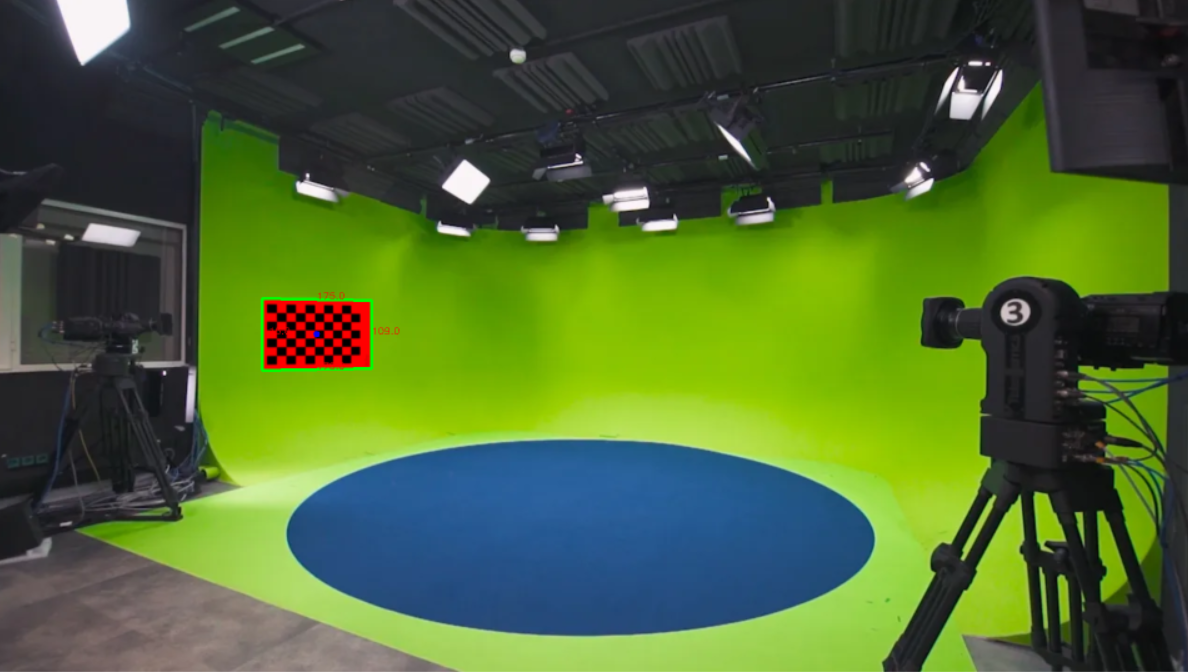
\includegraphics[width=\textwidth]{Images/04calibration/6.png}
        \caption{}
        \label{fig:a1}
    \end{subfigure}
    \hfill
    \begin{subfigure}[b]{0.45\textwidth}
        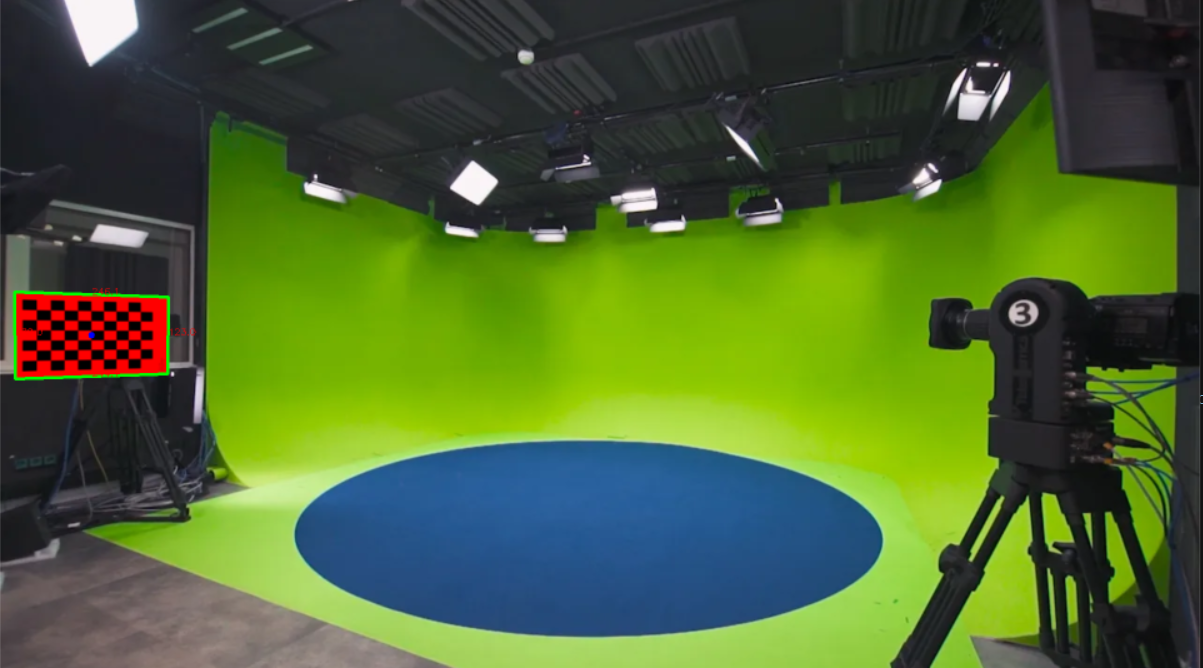
\includegraphics[width=\textwidth]{Images/04calibration/7.png}
        \caption{}
        \label{fig:b1}
    \end{subfigure}
    
    \vspace{0.5cm}
    
    \begin{subfigure}[b]{0.45\textwidth}
        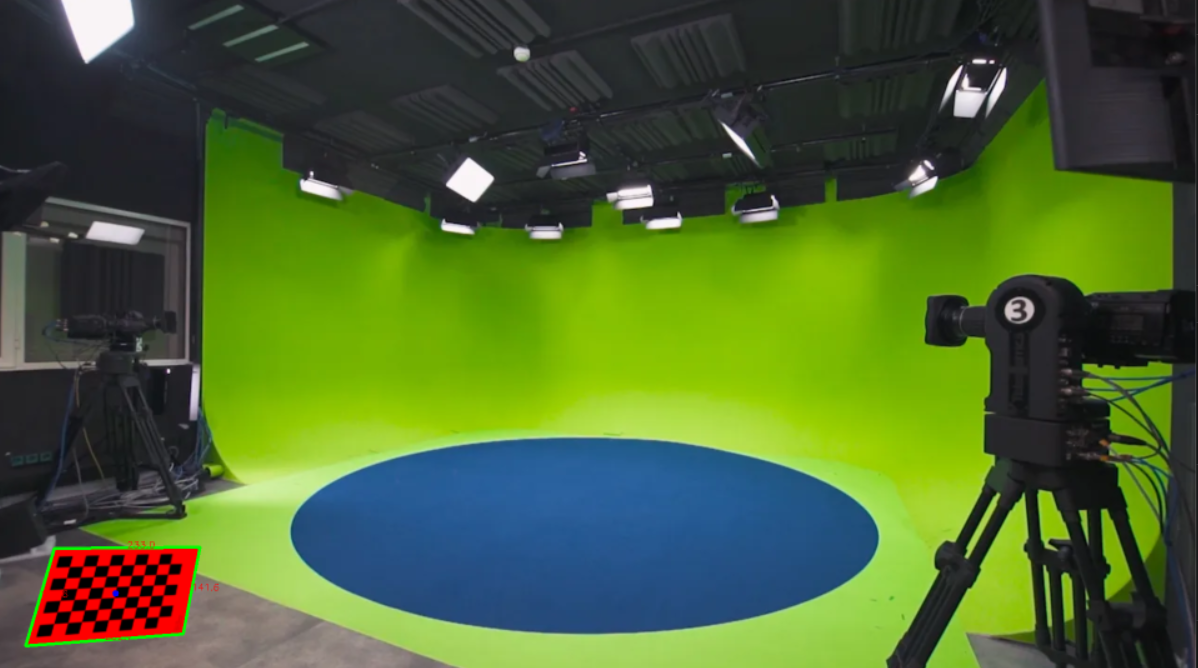
\includegraphics[width=\textwidth]{Images/04calibration/8.png}
        \caption{}
        \label{fig:c1}
    \end{subfigure}

    \caption{Example of K1, K2 and \ac{FoV} calibration using edge detection to determine the real object corners coordinates: (a) - \ac{FoV} calibration, (b) - K1 calibration, (c) - K2 calibration.}
    \label{fig:fov_cal}
\end{figure}

\begin{figure}[h]
    \centering
    \begin{subfigure}[b]{0.45\textwidth}
        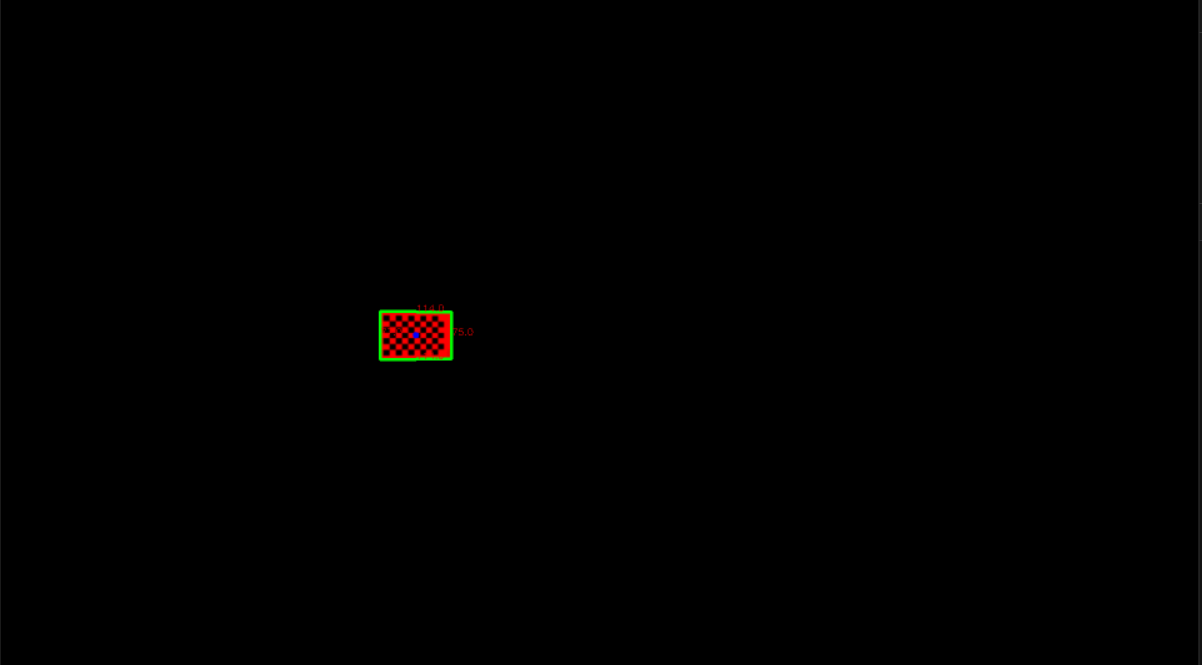
\includegraphics[width=\textwidth]{Images/04calibration/9.png}
        \caption{}
        \label{fig:a2}
    \end{subfigure}
    \hfill
    \begin{subfigure}[b]{0.45\textwidth}
        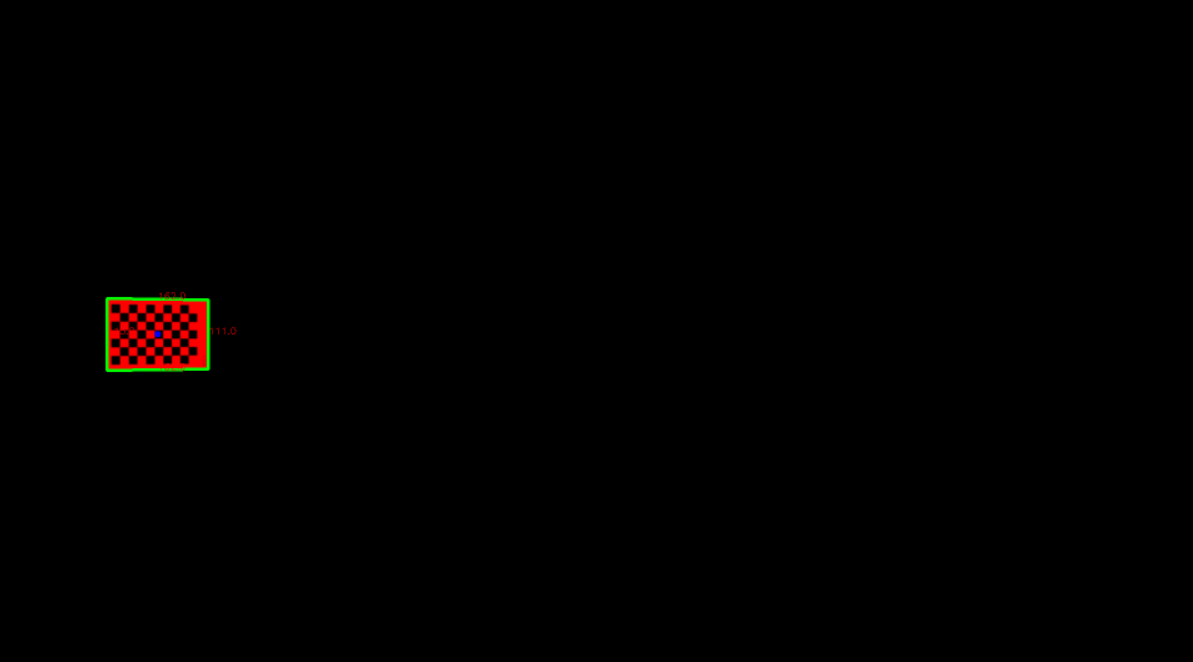
\includegraphics[width=\textwidth]{Images/04calibration/10.png}
        \caption{}
        \label{fig:b2}
    \end{subfigure}
    
    \vspace{0.5cm}
    
    \begin{subfigure}[b]{0.45\textwidth}
        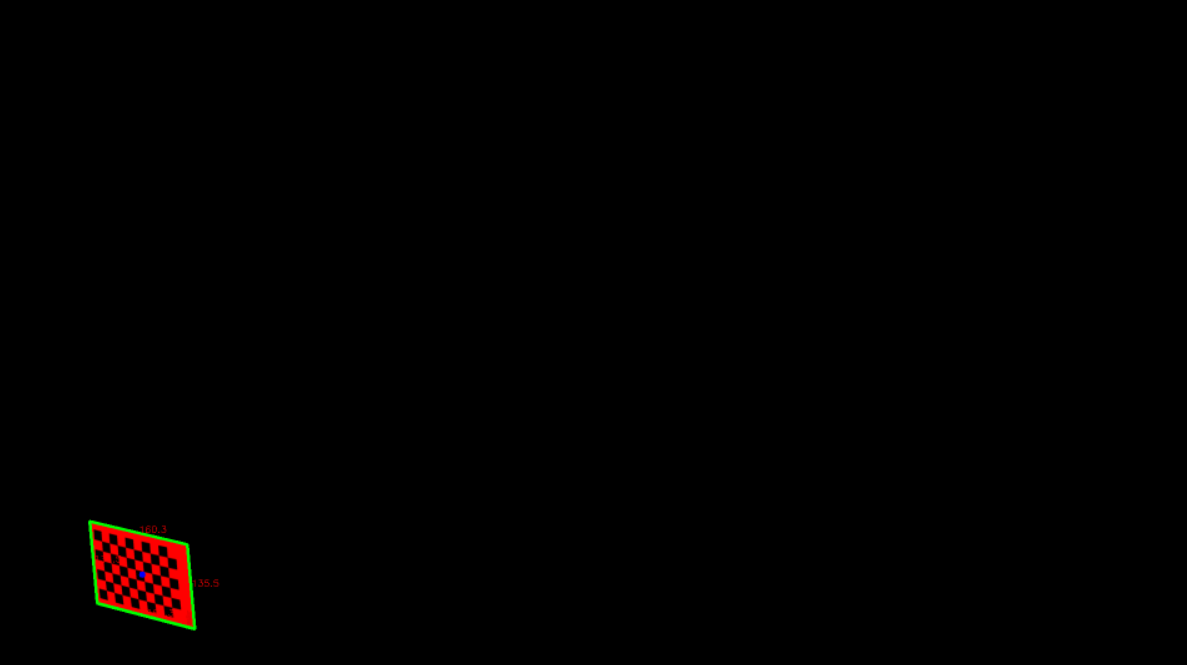
\includegraphics[width=\textwidth]{Images/04calibration/11.png}
        \caption{}
        \label{fig:c2}
    \end{subfigure}

    \caption{Example of K1, K2 and \ac{FoV} calibration using edge detection to determine the virtual object corners coordinates: (a) - \ac{FoV} calibration, (b) - K1 calibration, (c) - K2 calibration.}
    \label{fig:vir_fov_cal}
\end{figure}




\section{Calibration Scenarios} \label{sec:Calibration Scenarios}

\noindent The calibration process using the algorithm follows the same principles as manual calibration. First, it calibrates the \ac{FoV} to the best possible value. Then, it calibrates the K1 coefficient, iteratively refining both until they reach their optimal values. Afterward, the K2 calibration is performed using a similar iterative approach, adjusting both K1 and K2 until they are optimally calibrated.

\noindent After completing these steps, the algorithm’s results could be categorized into three scenarios:

\begin{itemize}
    \item \textbf{Scenario 1:} The \ac{FoV} and K1 are correctly calibrated, and K2 is extremely close to 0. In this case, the effect of K2 is negligible. To optimize time efficiency, the algorithm is modified to stop if the K1 and \ac{FoV} coefficients are already correctly calibrated. This is the most common scenario in real-world applications at most levels of calibration.
    
    \item \textbf{Scenario 2:} The K1 and \ac{FoV} are not correctly determined, indicating that the K2 coefficient is not negligible. In this case, the algorithm proceeds to calibrate the K2 coefficient.
    
    \item \textbf{Scenario 3:} After calibrating the K2 coefficient, if the K1 and K2 coefficients are still not correctly calibrated, the algorithm may have become stuck, recalibrating to the same values repeatedly. To resolve this issue, the algorithm is modified to detect this scenario and forcibly adjust the K1 value before recalibrating K2 until both coefficients are correctly calibrated.
\end{itemize}

\noindent The program effectively determines the distortion coefficients with satisfactory accuracy. However, the calibration process is time-consuming, taking approximately 65 minutes to complete six levels, which is impractical for efficient operation. In the next chapter, we will explore strategies to optimize and reduce the calibration time.

\section{Results} \label{sec:Results}

\begin{figure}[ht]
    \centering
    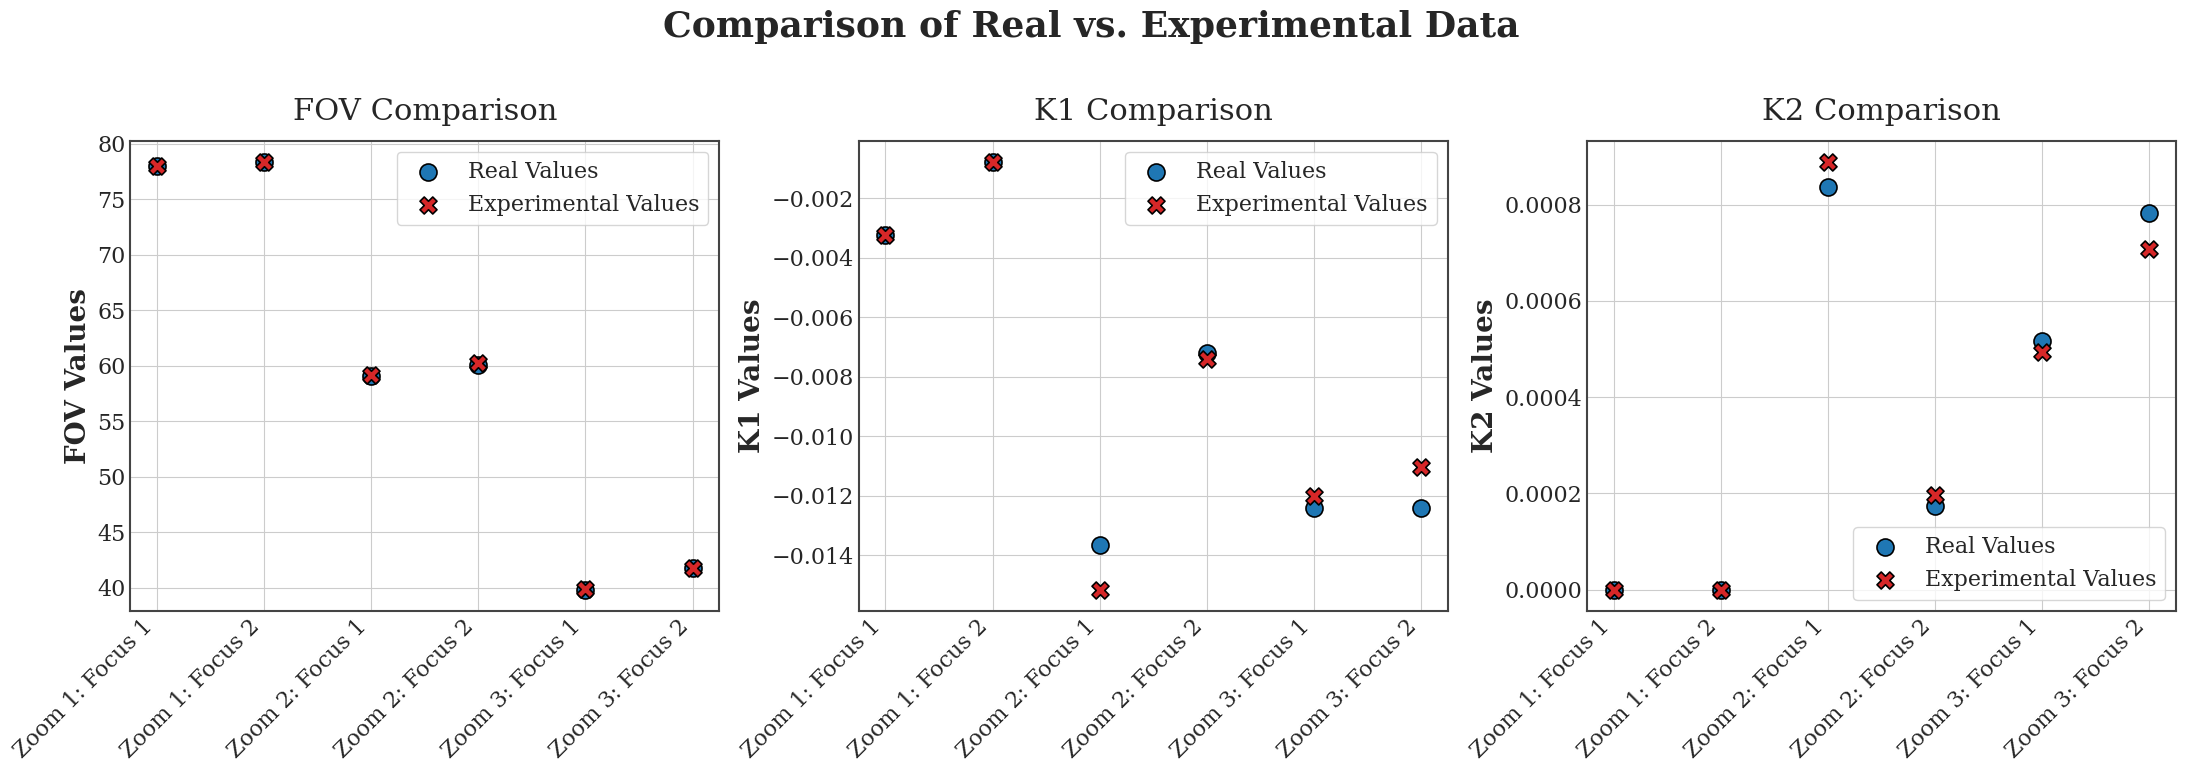
\includegraphics[width=1.1\textwidth]{Images/04calibration/novos_resul.png}
    \caption{Distortion calibration results}
    \label{fig:distortion}
\end{figure}




